A continuación se estima en horas hombre los módulos de nivel 1 y 2 del WBS. La estimación se basa en un grupo de trabajo de 4 recursos de 8 horas cada uno, 20 días por mes. Las horas hombre son las horas totales a consumir entre los 4 recursos sumados. Al final se realiza una sumarización de los números para estimar la duración total del proyecto.

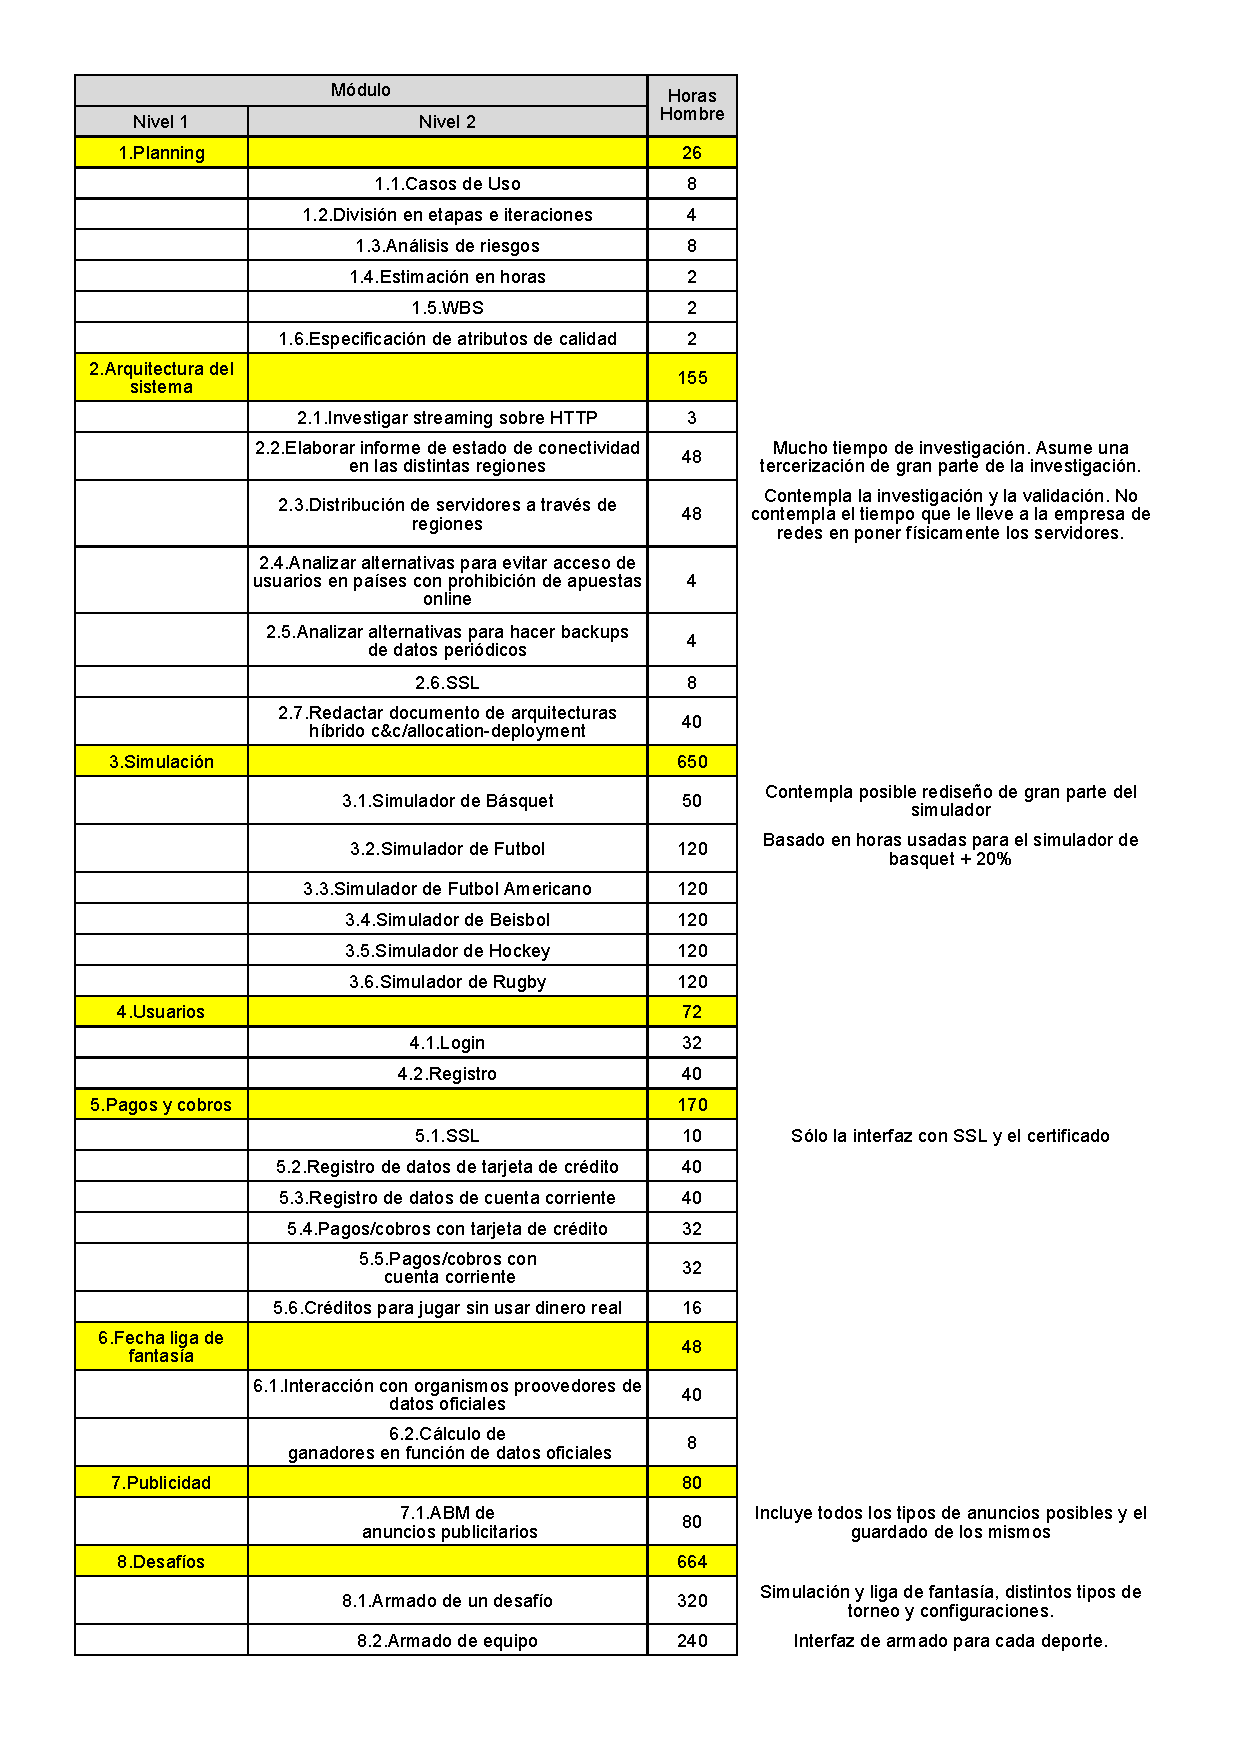
\includegraphics[width=\textwidth, page=1, clip, trim=20 0 20 30]{imagenes/estimacionModulos.pdf}

\newpage
\includegraphics[width=\textwidth, page=2, clip, trim=20 200 20 30]{imagenes/estimacionModulos.pdf}

Como puede observarse, el total estimado es bastante razonable para la magnitud del proyecto. Los tiempos podrían acelerarse si se contratara más gente y se tuviera un grupo de trabajo de 2 o 3 personas en cada módulo. Se estima que en 5 meses el proyecto debería estar funcionando, salvando las demoras que puedan causar los proveedores en responder y realizar su trabajo.